\documentclass{magnolia}

\magtex{tex_driver={pdftex},
        tex_packages={siunitx}}
\magfiche{document_nom={Cours sur les nombres complexes},
          auteur_nom={François Fayard},
          auteur_mail={fayard.prof@gmail.com}}
\magcours{cours_matiere={maths},
          cours_niveau={mpsi},
          cours_chapitre_numero={1},
          cours_chapitre={TP Python}}
\magmisenpage{}
\maglieudiff{}
\magprocess

\begin{document}

% https://pythonsandbox.com/turtle

%BEGIN_BOOK
\section{Découverte de Python}


\subsection{Les entiers}

\begin{questions}
\question Utiliser Python pour calculer $2022 + 2$, $2^{10}$, $3^2-2^3$.
\question Prédire avant de vérifier avec Python les résultats des opérations suivantes.
  \begin{center}
  \verb_10 // 2_, $\qquad$\verb_11 // 3_, $\qquad$\verb_-5 // 2_, $\qquad$\verb_11_ \% \verb_3_, $\qquad$\verb_-5_ \% \verb_2_
  \end{center}
\question Calculer $2^{\p{3^2}}$, puis $\p{2^3}^2$.
\question Afficher les nombres de Mersenne premiers suivants.
  \[2^3-1,\quad 2^7-1,\quad 2^{31}-1,\quad 2^{127}-1,\quad 2^{8191}-1,\quad 2^{131071}-1.\]
	% ,\quad 2^{524287}-1, \quad 2^{2147483647}-1\]
\end{questions}
%

\subsection{Les flottants}

\begin{questions}
\question Prédire puis vérifier le résultat des calculs suivants.
  \begin{center}
  \verb_0.1 + 0.2_, $\qquad$\verb_1.0 / 3.0_, $\qquad$\verb_0.5**3_.
  \end{center}
  Expliquer le premier résultat.
\question Calculer
  \begin{center}
  \verb_2 * 3.14159_, $\qquad$\verb_1 / 3_.
  \end{center}
\question En utilisant le fait que la vitesse de la lumière est de $c \approx 3.0\times 10^{8}\ {\rm m}.{\rm s}^{-1}$ et que la distance $d$ entre le soleil et la terre est de $d \approx 1.5\times 10^{11}\ {\rm m}$, déterminer le temps qu'il s'écoule avant que la lumière émise par le soleil arrive à la terre.
\question La distance moyenne entre 2 molécules d'eau liquide est de $3.4\times 10^{-10}\ {\rm m}$. Sachant qu'une mole contient de l'ordre de $6.0\times 10^{23}$ particules, donner un ordre de grandeur du nombre de moles dans un litre d'eau liquide.
\question À l'aide des fonctions du module \verb!math!, calculer
  \[\frac{1+\sqrt{5}}{2}, \quad \cos\p{\frac{\pi}{3}}, \quad \cos(\pi), \quad \sin(\pi), \quad\ln(2), \quad \log_{10}\p{1+\frac{1}{3}},\quad \e^{\pi\sqrt{163}}.\]
  Expliquer pourquoi l'un de ces résultats est surprenant.
\question Calculer puis expliquer le résultat des calculs suivants.
  \[(1 + 10^{-15}) - 1, \qquad (1 + 10^{-16}) - 1, \qquad (0.1 + 0.2) - 0.3, \qquad 0.1 + (0.2 - 0.3)\]
  On retiendra que les erreurs d'arrondis font que l'addition sur les nombres flottants n'est pas associative.
\question Prévoir, puis vérifier le type de
  \begin{center}
  \verb_5 // 2_, \quad \verb_5 / 2_, \quad \verb_(1 + math.sqrt(5)) / 2_, \quad \verb_4 / 2_
  \end{center}
\enonce Python permet de manipuler directement les nombres complexes. Le langage adopte les notations utilisées en physique~: le $\ii$ mathématique est noté $\jj$. Les nombres complexes en Python fonctionnent de la même manière que les nombres flottants. Le langage stocke la partie réelle et sa partie imaginaire comme des nombres flottants. Le nombre $2+\ii$ est entré sous la forme \verb_2+1j_.
\question Calculer $(2+\ii)(3+\ii)$.
\end{questions}

\subsection{Variables}

\begin{questions}
\question Quelle valeur contient la variable \verb_a_ après avoir écrit \verb_a = 1_ et exécuté 9 fois l'instruction \verb_a = 2 * a_~?
\question On considère les instructions suivantes
\begin{pythoncode}
In [1]: a = 1
In [2]: b = a
In [3]: c = b
In [4]: b = b + 1
\end{pythoncode}
Prévoir les valeurs de \verb_a_, \verb_b_ et \verb_c_ après l'exécution de ces instructions. Vérifier ensuite votre prédiction avec l'interpréteur Python.
\question À l'aide d'une troisième variable \verb_c_, échanger le contenu des variables \verb_a_ et \verb_b_.
\end{questions}

% \subsection{La méthode de Héron}

% La méthode de Héron est une méthode historique pour obtenir une valeur
% approchée de la racine carrée d'un nombre $a>0$. Pour cela, on définit la suite $(u_n)$ par
% \[u_0\defeq a, \quad\et\quad \forall n\in\N\qsep u_{n+1}\defeq\frac{u_n + \frac{a}{u_n}}{2}.\]
% Déterminer la plus petite valeur de $n$ pour laquelle la précision sur les nombres
% flottants ne permet plus de distinguer $u_{n+1}$ de $u_n$ lors du calcul de $\sqrt{2}$.

\section{Un peu de Logo}

Ce qu'on appelle aujourd'hui les graphismes \og tortue \fg trouvent leur origine dans le langage Logo, inventé dans
les années 1960 dans un but pédagogique. Ce langage comportait un certain nombre d'instructions qui permettaient de commander
un robot pouvant tracer des lignes sur une feuille de papier. La forme de ce robot, qui évoquait vaguement une tortue, a donné
son nom à cette manière de produire des dessins. Le module turtle de Python implémente une tortue virtuelle qui reproduit les
déplacements de son ancêtre dans une fenêtre de l'écran de votre ordinateur. C'est par son intermédiaire que nous allons
découvrir quelques concepts de base de la programmation. Dans le shell, tapez l'instruction suivante~:

\begin{pythoncode}
In [1]: import turtle as lg
In [2]: lg.reset()
\end{pythoncode}
\noindent
Une nouvelle fenêtre doit apparaitre à l'écran. Elle est peut-être cachée par Pyzo, donc redimensionnez votre espace de
travail afin de pouvoir visualiser en même temps l'éditeur, le shell et cette nouvelle fenêtre. Celle-ci représente
la feuille sur laquelle la tortue, représentée par défaut par la pointe d'une flèche, va réaliser ses dessins. Initialement
la tortue est située au point de coordonnées $(0, 0)$ situé au centre de la feuille et est orientée vers l'est, qui
correspond à un angle de $\ang{0}$. On rappelle les fonctions essentielles de la tortue~:

\begin{itemize}
\item \verb!lg.forward(c)! permet à la tortue d'avancer d'une distance de $c$.
\item \verb!lg.left(a)! permet à la tortue de tourner vers la gauche d'un angle de $a$ degrés.
\item \verb!lg.right(a)! permet à la tortue de tourner vers la droite d'un angle de $a$ degrés.
\item \verb!lg.reset()! permet de remettre à zéro le contenu de la fenêtre graphique.
\end{itemize}

\begin{questions}
\question Remettre à zéro le contenu de la fenêtre graphique, puis faire dessiner par la tortue un carré de côté 100 en tournant vers la gauche.
\enonce On souhaite désormais reproduire le dessin de la figure suivante.
\begin{center}
  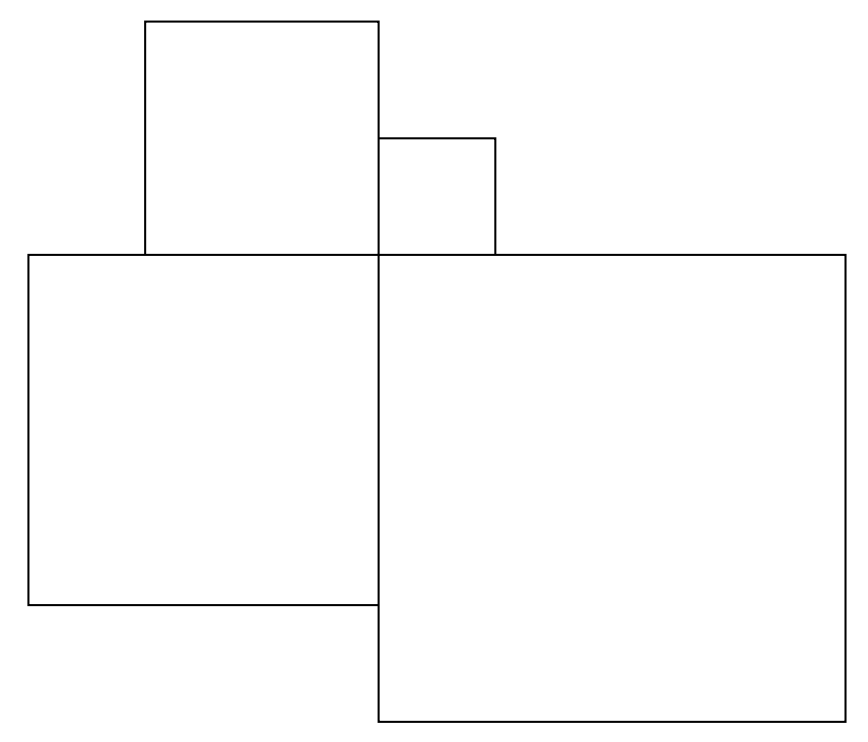
\includegraphics[width=0.4\textwidth]{../../Commun/Images/python-tp-logo-1}\\
  \textsc{Figure 1}
  \end{center}
Il pourrait être utile de disposer d'une fonction dessinant un carré de taille $c$. Puisqu'il n'existe pas de
telle fonction, nous allons la définir. Afin de définir une fonction, il faut lui donner un nom, préciser la
liste de ses paramètres et enfin décrire les différentes instructions à réaliser. La syntaxe générale est
la suivante.
\begin{pythoncode}
def (*@\textcolor{purple}{nom\_fonction}@*)((*@\textcolor{purple}{arg1, ..., argn}@*)):
    (*@\textcolor{purple}{bloc....................}@*)
    (*@\textcolor{purple}{..........d'instructions}@*)
\end{pythoncode}
Attention de bien respecter la syntaxe de l'instruction \verb!def!. La ligne contenant cette instruction
doit obligatoirement se terminer par un double point, et le bloc d'instructions qui suit doit être indenté,
c'est-à-dire décalé vers la droite de 4 espaces. Heureusement, si vous n'avez pas fait d'erreur de syntaxe,
l'éditeur de code se chargera pour vous d'indenter automatiquement votre code. Par exemple, pour
définir la fonction qui nous intéresse et que nous allons nommer \verb!carre! et qui dessine un carré de côté
$c$ en tournant vers la gauche, on commencera par écrire
\begin{pythoncode}
def carre(c):
    (*@\textcolor{purple}{bloc....................}@*)
    (*@\textcolor{purple}{..........d'instructions}@*)
\end{pythoncode}
\question Achever la définition de la fonction \verb!carre(c)! en prenant soin à ce que la tortue regarde dans
  la même direction qu'au début une fois le tracé effectué. Puis, à l'aide de celle-ci, reproduire le dessin de la
  figure 1, où les carrés ont respectivement pour côté 50, 100, 150 et 200. On écrira pour cela une fonction \verb!figure1()!.
\enonce Nous allons maintenant chercher à reproduire le dessin de la figure suivante.
\begin{center}
  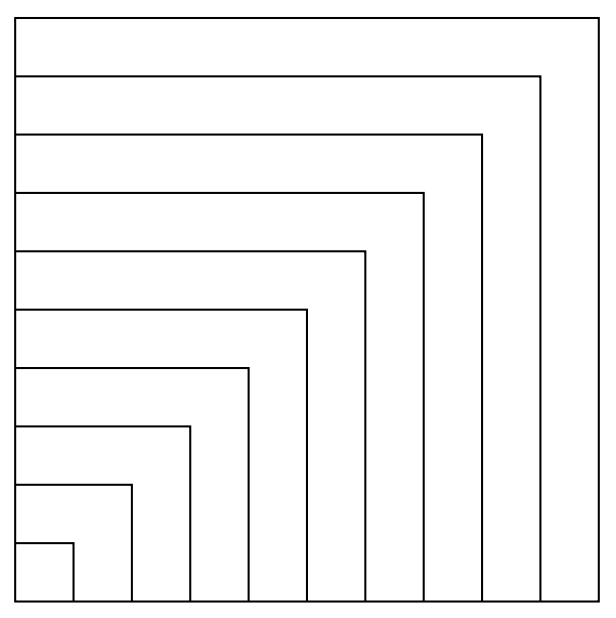
\includegraphics[width=0.3\textwidth]{../../Commun/Images/python-tp-logo-2}\\
  \textsc{Figure 2}
  \end{center}
  À l'aide de la fonction \verb!carre!, le script n'est pas difficile à réaliser, mais peut s'avérer
  fastidieux à écrire. Pour en faciliter l'écriture, nous allons introduire la notion de boucle. Si
  $a$ et $b$ sont deux entiers, le script
\begin{pythoncode}
for k in range(a, b):
    (*@\textcolor{purple}{bloc....................}@*)
    (*@\textcolor{purple}{..........d'instructions}@*)
\end{pythoncode}
va exécuter le bloc d'instruction en utilisant successivement $a, a+1, \ldots, b - 1$ pour valeur de $k$.
\question À l'aide d'une boucle, écrire une fonction
  \verb!figure2(c)! qui reproduit le dessin de la figure 2 où les carrés ont
  pour côtés respectifs $c, 2c, 3c, \ldots, 10c$.
\enonce Effacer l'écran, puis augmenter la vitesse de la tortue jusqu'à sa vitesse maximale, car le dessin
  qui va suivre va être un peu long à tracer. Pour cela, on utilisera la fonction \verb!lg.speed(s)! avec
  pour valeur de $s$ un entier compris entre 1 (lent) et 10 (rapide); la valeur 0 permet aussi d'obtenir la vitesse la plus rapide. Attention, en
  plus d'effacer l'écran, la commande \verb!lg.reset()! rétablit la vitesse d'origine.
\question Écrire une fonction \verb!tourne(n)! qui, à l'aide d'une boucle, fait avancer la tortue de 1, puis de $2, 3, 4, \ldots, n$ pas en
  tournant d'un angle de \ang{91} entre chaque déplacement. Une fois
  la vitesse réglée au maximum, on pourra faire un essai avec
  \verb!tourne(500)!.
\question Tracer un triangle équilatéral, un carré, un pentagone ou un hexagone régulier ne sont
  pas des tâches fondamentalement différentes. Définir une fonction \verb!polygone(n, c)! qui
  trace un polygone régulier à $n$ côtés, chacun de longueur $c$, puis reproduire à l'aide de cette
  fonction la figure 3.
\begin{center}
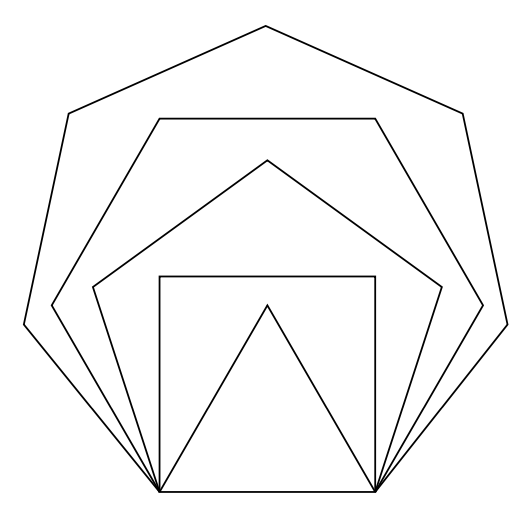
\includegraphics[width=0.3\textwidth]{../../Commun/Images/python-tp-logo-3}\\
\textsc{Figure 3}
\end{center}
\enonce Effacer de nouveau l'écran à l'aide de la fonction \verb!lg.reset()!, puis réaliser la commande
  \verb!polygone(100, 5)!. La courbe obtenue vous étonne-t-elle~? Elle peut aussi être obtenue à l'aide
  d'une fonction prédéfinie du module \verb!turtle! qui se nomme \verb!circle!, mais dont les
  paramètres sont différents. Pour en connaitre les spécifications, vous pouvez chercher les mots-clés
  \verb!turtle python! avec votre moteur de recherche internet et vous diriger vers le site \verb!docs.python.org!.
  Vous constaterez que cette fonction possède trois arguments, dont deux optionnels. Le second, \verb!extent!,
  lorsqu'il est présent, permet de tracer un arc de cercle plutôt qu'un cercle complet. Le troisième,
  \verb!steps!, permet de tracer des polygones.
\question Écrire une fonction \verb!figure4()! qui, à l'aide de la seule fonction \verb!circle!, permet de reproduire le dessin de la figure 4. Une commande
  permet de tracer le cercle et c'est une utilisation astucieuse de la
  fonction \verb!circle! qui permet de tracer l'étoile.
  \emph{Si vous ne trouvez pas rapidement, passez à la question suivante.}
\begin{center}
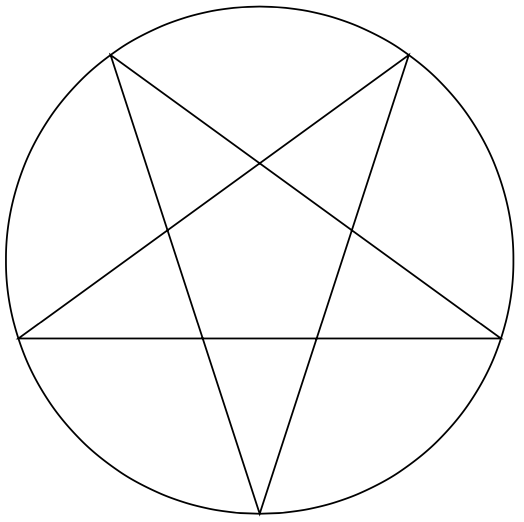
\includegraphics[width=0.3\textwidth]{../../Commun/Images/python-tp-logo-4}\\
\textsc{Figure 4}
\end{center} 
\question Écrire enfin une fonction \verb!figure5()! permettant de reproduire
  le dessin de la figure 5. Ce dernier est constitué de 72 demi-cercles
  régulièrement espacés. Avant de tracer cette figure, il pourra être utile d'accélérer la vitesse de la tortue
  pour éviter une attente trop longue.
\begin{center}
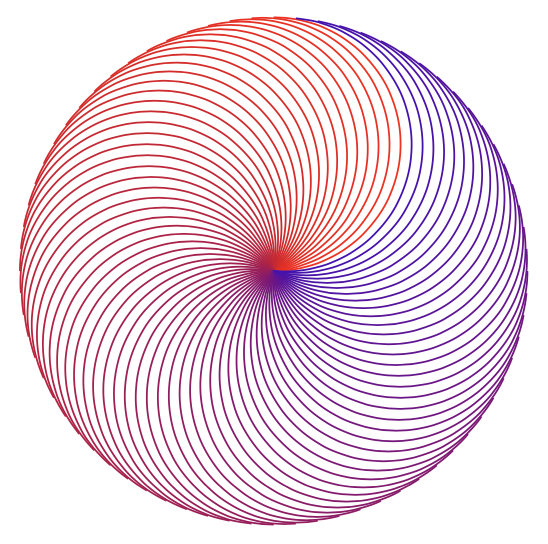
\includegraphics[width=0.3\textwidth]{../../Commun/Images/python-tp-logo-5}\\
\textsc{Figure 5}
\end{center}
\enonce Le triangle de Sierpi\'nski est une fractale qui s'obtient à partir d'un triangle plein par une infinité de
  répétitions consistant à diviser par 2 la taille du triangle puis à les accoler en trois exemplaires par leurs
  sommets pour former un nouveau triangle. On trouvera figure 6 la représentation graphique des trois premières
  générations de cette transformation.
\begin{center}

\includegraphics[width=0.6\textwidth]{../../Commun/Images/python-tp-logo-6}\\
\textsc{Figure 6}
\end{center}
Pour colorier l'intérieur d'une courbe fermée, il faut faire précéder le début du tracé par la commande
\verb!lg.begin_fill()! et terminer celui-ci par \verb!lg.end_fill()!. Par exemple, le script suivant
\begin{pythoncode}
lg.begin_fill()
lg.circle(100)
lg.end_fill()
\end{pythoncode}
crée un disque plein.
\question Définir une fonction \verb!sierp1(c)! qui dessine la première étape de la construction du triangle
  de Sierpi\'nski, c'est-à-dire un triangle plein de côté $c$, en prenant soin à ce que la tortue regarde dans
  la même direction qu'au début une fois le tracé effectué.
\question À l'aide de la fonction précédente, définir une fonction \verb!sierp2(c)! qui dessine la deuxième
  étape de la construction du triangle de Sierpi\'nski.
\question À l'aide de la fonction précédente, définir une fonction \verb!sierp3(c)! qui dessine la troisième
  étape de la construction du triangle de Sierpi\'nski.
\enonce Les questions précédentes ont du vous convaincre qu'à l'exception de la première, la $n^e$ génération
  du triangle de Sierpi\'nski s'exprime toujours de la même manière en fonction de la précédente. Pour exploiter
  cette remarque, nous allons utiliser une particularité des fonctions Python~: elles ont la possibilité de
  faire appel à elle-mêmes dans leur définition. Autrement dit, si nous choisissons de passer en paramètre l'ordre
  $n$ de la génération que nous voulons tracer en définissant une fonction \verb!sierpinski(n, c1)!, il est possible,
  au sein de cette définition, de faire appel à la fonction \verb!sierpinski(n - 1, c2)!. Mais pour cela, il faut
  distinguer le cas $n=1$ qui se traite différemment. Pour effectuer cette distinction, on utilise l'instruction
  conditionnelle \verb!if! dont la syntaxe est la suivante~:
\begin{pythoncode}
if test:
    (*@\textcolor{purple}{bloc....................}@*)
    (*@\textcolor{purple}{........d'instructions 1}@*)
else:
    (*@\textcolor{purple}{bloc....................}@*)
    (*@\textcolor{purple}{........d'instructions 2}@*)
\end{pythoncode}
Notez bien l'indentation qui permet de délimiter chacun des deux blocs d'instructions. Le fonctionnement de
cette instruction est le suivant~: si le résultat du test est positif, le premier bloc d'instruction est
réalisé. Dans le cas contraire, c'est le second. Notez que l'instruction \verb!else! est optionnelle si aucune
instruction de doit être réalisée dans le cas d'un test négatif. 
\question Écrire la fonction \verb!sierpinski(n, c)! qui dessine la génération d'ordre $n$ du triangle de
  Sierpi\'nski avec une longueur de côté égale à $c$. Utiliser ensuite cette fonction pour effectuer le tracé
  avec $n=5$. N'oubliez pas d'accélérer au maximum la vitesse de la tortue car sinon, le tracé sera très long.
\enonce D'autres structures fractales peuvent être dessinées par la tortue, à commencer par l'arbre binaire
  représenté figure 7. Pour construire l'arbre d'ordre $n$ et de hauteur $h$, on procède de la manière
  suivante~:
  \begin{itemize}
  \item On trace le tronc de hauteur $h/3$ et d'épaisseur $n$.
  \item Puis on trace ses deux branches, qui sont des arbres d'ordre $n-1$ et de hauteur $2h/3$, inclinés
    d'un angle de \ang{30}.
  \end{itemize}
\begin{center}
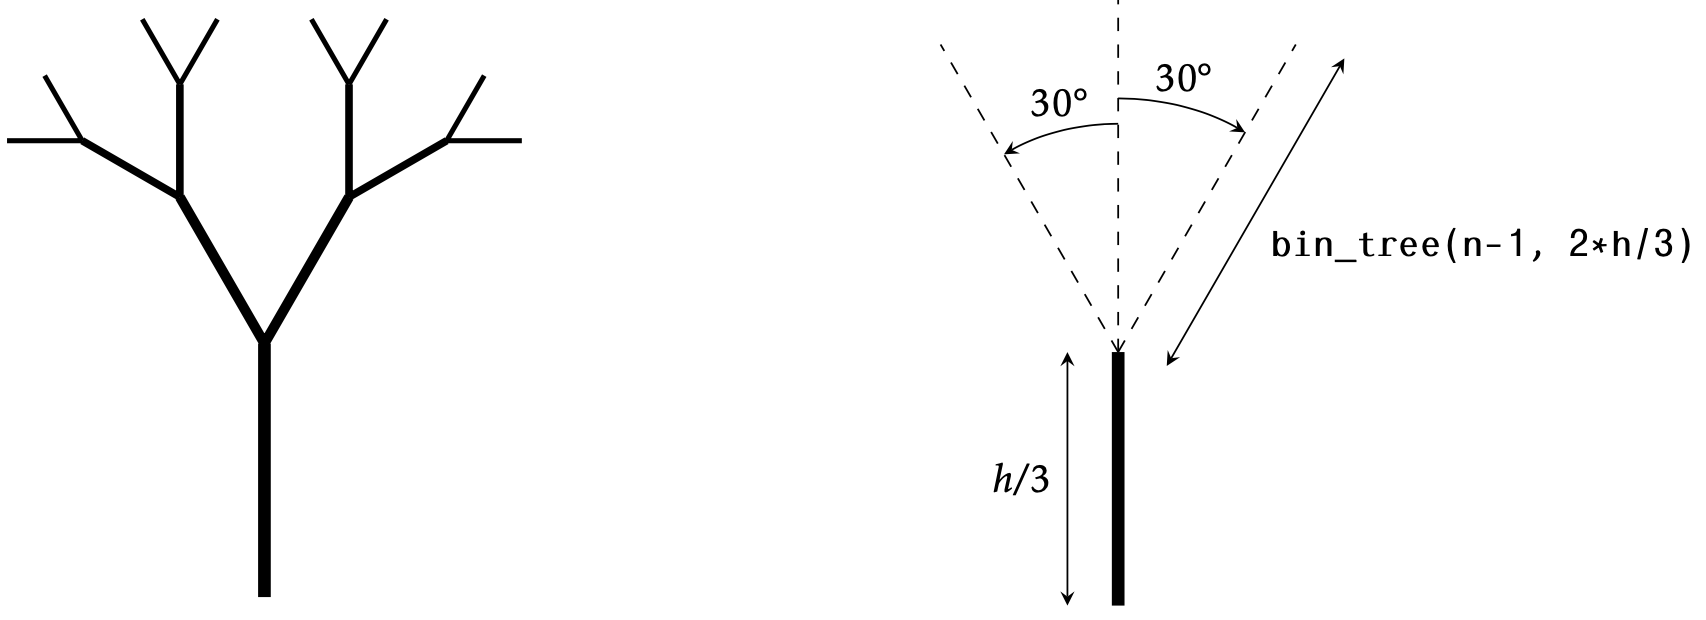
\includegraphics[width=0.6\textwidth]{../../Commun/Images/python-tp-logo-7}\\
\textsc{Figure 7} -- L'arbre d'ordre $n=4$ et sa règle de construction
\end{center}
\question Définir une fonction \verb!bin_tree(n, h)! qui dessine l'arbre binaire d'ordre $n$ et de hauteur $h$,
  puis dessiner l'arbre d'ordre 8.
\end{questions}

% \subsection{Noeud papillon}

% Tracez en \textsc{logo} le noeud papillon suivant. La hauteur du noeud papillon est de
% 100 et sa largeur est de 200. On utilisera la fonction \verb_atan(theta: float) -> float_ du module
% \verb_math_ qui calcule la mesure $\theta\in\intero{-\pi/2}{\pi/2}$ en radian de
% l'unique angle dont la tangente vaut $x$.
% \begin{center}
% \includegraphics[width=0.25\textwidth]{../../Commun/Images/python-exos-val-1.pdf}
% \end{center}


% \subsection{Suites récurrentes}

% Étant donnés $\alpha,\beta\in\RP$, on définit les suites $(a_n)$ et $(b_n)$ par
% \[a_0\defeq\alpha\qsep b_0\defeq\beta\qsep\et\quad \cro{
% 	\forall n\in\N\qsep a_{n+1}\defeq\frac{a_n+b_n}{2}\quad\et\quad b_{n+1}\defeq\sqrt{a_n b_n}}.\]
% \begin{questions}
% \question On suppose que les variables \verb!a! et \verb!b! contiennent respectivement
%   les valeurs $a_n$ et $b_n$. Écrire un code Python tel qu'après
% 	l'execution de ce code, les variables \verb!a! et \verb!b! contiennent respectivement
%   les valeurs $a_{n+1}$ et $b_{n+1}$.
% \question On suppose que $\alpha=1.0$ et que $\beta=2.0$. Quelle est la plus petite valeur
%   de $n$ pour laquelle la précision du type \verb!float! ne permet plus de discerner $a_n$
% 	de $b_n$~?
% \end{questions}
% \begin{sol}
% On trouve $n=4$.
% \end{sol}


% \section{Fonction, flot d'execution}

% \subsection{Boucle for}

% \begin{questions}
% \question  Écrire une fonction \verb+somme_cube(n: int) -> int+ calculant la somme des cubes de entiers
%   allant de 0 à $n$.
% \question Écrire une fonction \verb+somme_3_5(n: int) -> int+ calculant la somme de tous les
%   entiers inférieurs ou égaux à $n$ qui sont multiples de 3 ou de 5.
% \question Écrire une fonction \verb_factorielle(n: int) -> int_ calculant $n!$.
% \question
%   \begin{questions}
% 	\question Écrire une fonction \verb_exponentielle(x: float, n: int) -> float_ calculant
%     \[\sum_{k=0}^n \frac{x^k}{k!}.\]
% 		Comparer \verb_exponentielle(x, n)_ et \verb_exp(x: float) -> float_ du module \verb_math_
% 		pour quelques valeurs de $x$ et de $n$.
% 	\question Essayer d'écrire cette fonction de manière efficace sans utiliser, ni la
% 	  fonction puissance, ni la fonction factorielle. 
% 	\end{questions}
% \question On définit la suite de \textsc{Fibonacci} par
%   \[F_0\defeq 0, \quad F_1\defeq 1, \et \forall n\in\N\qsep F_{n+2}\defeq F_{n+1}+F_n.\]
%   Écrire une fonction \verb_fibo(n: int) -> int_ calculant le $n$-ième terme de la suite de
% 	\textsc{Fibonacci}.

% \question Une tortue ivre avance de $n$ pas. Avant chaque pas, elle tourne d'un angle
%   choisi de manière aléaoire uniformément entre 0 et 360. Écrire une fonction
% 	\verb+tortue_ivre(pas: int, n: int) -> NoneType+ simulant une telle marche, le paramètre \verb_pas_
% 	désignant la longueur d'un pas de la tortue. On utilisera pour cela,
% 	après avoir importé le module \verb_random_, l'expression \verb_random.randrange(360)_
% 	qui renvoie un entier $\theta$ tel que $0\leq \theta< 360$.
% \begin{center}
% \includegraphics[width=0.1\textwidth]{../../Commun/Images/python-tps-valeur_flot-1.pdf}
% \end{center}
% % \question \textsc{John Von Neumann} a proposé le générateur (uniforme sur $\interf{0}{1}$) de nombres aléatoires suivant. On se donne une graine $x\in\interf{0}{1}$ et on définit la suite $(u_n)$ par
% %   \[u_0\defeq x \et \forall n\in\N\qsep u_{n+1}\defeq 4 u_n(1-u_n).\]
% % On définit ensuite la suite $(r_n)$ par
% % \[\forall n\in\N\qsep r_n\defeq\frac{\arccos(1-2u_n)}{\pi}.\]
% % Afin de vérifier la qualité de ce générateur $(r_n)$, écrire une fonction \verb_moyenne(x, n)_ calculant la moyenne des $n$ premiers nombres de cette suite ainsi que la fonction \verb_variance(x, n)_ calculant la variance de ces nombres.
% \question Écrire une fonction \verb+polygone(r: int, n: int) -> NoneType+ dessinant un polygone régulier 
%   à $n$ côtés inscrit dans un cercle de rayon $r$.
% \end{questions}



% \subsection{Constante d'\textsc{Euler}}

% On note pour tout $n \in \Ns$
% \[S_n\defeq \sum_{k=1}^{n} \frac{1}{k},\qquad
% 	u_n\defeq S_n-\ln(n) \et v_n\defeq u_n-\frac{1}{n}.\] 
% On admet que $(u_n)$ et $(v_n)$ tendent vers la même limite $\gamma$ appelée constante
% d'\textsc{Euler} et que l'on a
% \[\forall n \in\Ns \qsep v_n \leq \gamma \leq u_n.\]
% Écrire une fonction \verb_euler(eps: float) -> float_ qui calcule une approximation à $\epsilon$ près de $\gamma$.


% \subsection{Suite de \textsc{Conway}}

% Les premiers termes de la suite de \textsc{Conway} sont $1, 11, 21, 1211, 111221,\ldots$
% chaque terme étant obtenu en lisant à haute voix le terme précédent. C'est pourquoi
% \textsc{Conway} avait baptisé cette suite \emph{look and say}. Par exemple, le terme
% 1211 se lit \og un 1, un 2, deux 1\fg donc le terme suivant est 111221.
% \begin{questions}
% \question Écrire une fonction \verb!look_and_say(s: string)! prenant en paramètre une chaîne de
%   caractères représentant un entier et renvoyant la chaîne de caractère représentant
% 	l'entier suivant dans la suite de \textsc{Conway}.
% \question À l'aide de cette fonction, afficher les 20 premiers termes de la suite de
%   \textsc{Conway}.
% \question Il a été démontré que si on note $u_n$ le nombre de chiffres du $n$-ième
%   nombre de \textsc{Conway}, le rapport $u_{n+1}/u_n$ admet une limite finie $l$.
% 	Donnez une valeur approchée de $l$.
% \question Une autre propriété de cette limite est qu'elle ne dépend pas de la
%   valeur initiale (excepté 22). Le vérifier expérimentalement.
% \question Démontrer que dans a suite de \textsc{Conway}, ne peuvent apparaître que les chiffres 1, 2 et 3.
% \end{questions}

%END_BOOK
\end{document}